\chapter{Perturbation Theory and Gravitational Radiation}
\section{The linearized theory of gravity}
In a weak-field situation
\[g_{\mu\nu} = \eta_{\mu\nu} + h_{\mu\nu} , \quad |h_{\mu\nu}| \ll 1 ,\]
one can expand the field equations in powers of $h_{\mu\nu}$ using a coordinate frame where $|h_{\mu\nu}| \ll 1$ holds; and without much loss of accuracy, one can keep only linear terms. The resulting formalism is often called ``the linearized theory of gravity''. The resulting connection coefficients, when linearized in the metric perturbation $h_{\mu\nu}$, read 
\[\Gamma^{\mu}_{\alpha \beta} = \frac{1}{2}\eta^{\mu\nu} (h_{\alpha\nu,\beta} + (h_{\beta\nu,\alpha} - h_{\alpha\beta,\nu}) \equiv \frac{1}{2}(h_{\alpha \phantom{*},\beta}^{\phantom{*} \mu} + h_{\beta \phantom{*},\alpha}^{\phantom{*} \mu} + h_{\alpha\beta}^{\phantom{**} ,\mu} ).\]
Whenever one expands in powers of $h_{\mu\nu}$, indices of $h_{\mu\nu}$ are raised and lowered using $\eta^{\mu\nu}$ and $\eta_{\mu\nu}$, not $g^{\mu\nu}$ and $g_{\mu\nu}$. A similar linearization of the Ricci tensor yields
\[R_{\mu\nu} = \Gamma^{\alpha}_{\phantom{*}\mu\nu,\alpha} - \Gamma^{\alpha}_{\phantom{*}\mu\alpha,\nu} = \frac{1}{2}(h_{\mu \phantom{*},\nu\alpha}^{\phantom{*} \alpha} + h_{\nu \phantom{*},\mu\alpha}^{\phantom{*} \alpha} - h_{\mu\nu,\alpha}^{\phantom{***}\alpha} - h_{,\mu\nu}),\]
where
\[h \equiv \eta_{\mu\nu}h^{\mu\nu}.\]
After a further contraction to form $R \equiv g^{\mu\nu}R_{\mu\nu} \approx \eta^{\mu\nu}R_{\mu\nu}$,
one finds the Einstein equations read
\[h_{\mu\alpha,\nu}^{\phantom{****}\alpha} + h_{\nu\alpha,\mu}^{\phantom{****}\alpha} - h_{\mu\nu,\alpha}^{\phantom{****}\alpha} - h_{,\mu\nu} - \eta_{\mu\nu}(h^{\alpha\beta}_{\phantom{**},\alpha\beta} - h_{,\alpha}^{\phantom{*}\alpha}) = 16\pi T_{\mu\nu}.\]
Define
\[\overline{h}_{\mu\nu} \equiv h_{\mu\nu} - \frac{1}{2}\eta_{\mu\nu}h.\]
The linearized field equations become
\[H^{\mu\alpha\nu\beta}_{\phantom{****},\alpha\beta} = 16\pi T_{\mu\nu},\]
where
\[-H^{\mu\alpha\nu\beta} \equiv \overline{h}^{\mu\nu}\eta^{\alpha\beta} + \overline{h}^{\alpha\beta}\eta^{\mu\nu} - \overline{h}^{\alpha\nu}\eta^{\mu\beta} - \overline{h}^{\mu\beta}\eta^{\alpha\nu} .\]
\\
Two different types of coordinate transformations connect nearly globally Lorentz systems to each other: global Lorentz transformations, and infinitesimal coordinate
transformations.
\\
Global Lorentz Transformations:
\\
\[x^{\mu} = \Lambda^{\mu}_{\phantom{*}\alpha'}x^{\alpha'} , \quad \Lambda^{\mu}_{\phantom{*}\alpha'} \Lambda^{\nu}_{\phantom{*}\beta'} \eta_{\mu\nu} = \eta_{\alpha'\beta'} .\]
We can verify that $h_{\mu\nu}$ and $\bar{h}_{\mu\nu}$
transform like components of a tensor in flat spacetime
\[h_{\alpha'\beta'} = \Lambda^{\mu}_{\phantom{*}\alpha'} \Lambda^{\nu}_{\phantom{*}\beta'} h_{\mu\nu}.\]
Infinitesimal Coordinate Transformations:
\\
\[x^{\mu'} = x^{\mu} + \xi^{\mu},\]
where $\xi^{\mu}$ are four arbitrary functions small enough to leave $|h_{\mu'\nu'}| \ll 1$. We can verify that the metric perturbation functions in the new $x^{\mu'}$ and old $x^{\mu}$ coordinate systems are related by
\[h_{\mu\nu}^{\mathrm{new}} = h_{\mu\nu}^{\mathrm{old}} - \xi_{\mu,\nu} - \xi_{\nu,\mu},\]
whereas the functional forms of all other scalars, vectors, and tensors which is of order $O(h)$, such as $R_{\mu\nu}$, $T_{\mu\nu}$ and $R$, are unaltered, to within the precision of linearized theory. 
\\ \\
For any physical situation, one can specialize the gauge so that
\[\overline{h}^{\mu\alpha}_{\phantom{**},\alpha} = 0,\] 
called Lorentz gauge. 
The Lorentz gauge is not fixed uniquely. The gauge condition is left unaffected by any gauge transformation for which
\[\Box \xi \equiv \xi^{\alpha,\beta}_{\phantom{**}\beta} = 0.\]
The field equations then become
\[\Box h_{\mu\nu} = -16\pi T_{\mu\nu}.\]
Once the gauge has been fixed by fiat for a given system, one can regard $h_{\mu\nu}$ as components of tensors in flat spacetime; and one can regard the field equations and the chosen gauge conditions as geometric, coordinate-independent equations in flat spacetime.
This viewpoint allows one to use curvilinear coordinates, if one wishes. But in doing so, one must everywhere replace the Lorentz components of the metric $\eta_{\mu\nu}$ by the metric's components $g_{\mu\nu_{\mathrm{flat}}}$ in the flat-spacetime curvilinear coordinate system; and one must replace all ordinary derivatives in the field equations and gauge conditions by covariant derivatives whose connection coefficients come from $g_{\mu\nu_{\mathrm{flat}}}$.

\section{Nearly Newtonian gravitational fields}
The general solution to the linearized field equations in Lorentz gauge lends itself to expression as a retarded integral of the form familiar from electromagnetic theory:
\[\overline{h}_{\mu\nu}(t,\bm{x}) = \int \frac{4T_{\mu\nu}(t-r,\bm{x}')}{r} d^3x' , \quad r = |\bm{x}-\bm{x}'|.\]
Here focus attention on a nearly Newtonian source: $T_{00} \gg |T_{0i}|$ and $T_{00} \gg |T_{ij}|$, and velocities
slow enough that retardation is negligible. In this case, we have
\[\overline{h}_{00} = -4\Phi , \quad \overline{h}_{0i} = \overline{h}_{ij} = 0.\]
\[\Phi(t,\bm{x}) = -\int \frac{T_{00}(t,\bm{x}')}{r} d^3x' = \mbox{ Newtonian potential }.\]
The corresponding metric is
\[ds^2 = -(1+2\Phi)dt^2 + (1-2\Phi)(dx^2 + dy^2 + dz^2) \approx -(1-\frac{2M}{r})dt^2 + (1+\frac{2M}{r})(dx^2 + dy^2 + dz^2).\]
For a test particle whose velocity $v \ll 1$, the geodesic equation can be written as
\[\frac{d^2 v^i}{dt^2} + \Gamma^{i}_{00} = \frac{d^2 v^i}{dt^2} + \Phi_{,i} = 0.\]
Therefore, we reproduce the classical Newtonian gravitation theory.
\\ \\
Now let us consider the path of a photon through
this geometry; in other words, solve the perturbed geodesic equation for a null trajectory $x^{\mu}(\lambda)$. (We parametrize the trajectory with $\lambda$ to ensure that $p^{\mu} = dx^{\mu}/d\lambda$.)
Recall that our philosophy is to consider the metric perturbation as a field defined on a flat background spacetime. 
Similarly, we can decompose the geodesic into a background path plus a perturbation,
\[x^{\mu}(\lambda) = x^{(0)\mu}(\lambda) + x^{(1)\mu}(\lambda),\]
where $x^{(0)\mu}(\lambda)$ solves the geodesic equation in the background. 
We then evaluate all quantities along the background path, to solve for $x^{(1)\mu}(\lambda)$. 
For this procedure to make sense, we need to assume that the potential $\Phi$ is not appreciably different along the background and true geodesies;
this condition amounts to requiring that $x^{(1)i}\partial_{i}\Phi \ll \Phi$. 
For convenience we denote the wave vector of the background path as $k^{\mu}$ and the derivative of the deviation vector as $l^{\mu}$. The condition that a path be null is of course
\[(\eta_{\mu\nu} + h_{\mu\nu})(l^{\mu}+k^{\mu})(l_{\nu} + k_{\nu}) = 0.\]
At zeroth order we simply have
\[\eta_{\mu\nu} k^{\mu} k^{\nu} = 0.\]
i.e.
\[k^2 \equiv (k^0)^2 = \vec{k}\cdot\vec{k}.\]
At first order we obtain
\[2\eta_{\mu\nu}k^{\mu}l^{\nu} + h_{\mu\nu}k^{\mu}k^{\nu} = 0,\]
i.e.
\[-k l^0 + \vec{l}\cdot\vec{k} = 2k^2\Phi.\]
We now turn to the perturbed geodesic equation. The zeroth-order geodesic equation simply tells us that $x^{(0)\mu}(\lambda)$ is a straight  trajectory, while at first order we have
\[\frac{dl^{\mu}}{d\lambda} = -\Gamma^{\mu}_{\rho\sigma}k^{\rho}k^{\sigma},\]
i.e.
\[\frac{dl^0}{d\lambda} = -2k(\vec{k}\cdot\vec{\nabla}\Phi), \quad \frac{d\vec{l}}{d\lambda} = -2k^2\vec{\nabla}_{\bot}\Phi,\]
where $\vec{\nabla}_{\bot} \equiv k^{-2}\vec{k}(\vec{\nabla} - \vec{k}\cdot\vec{\nabla})$.
Putting all equations together, we have
\[l^0 = -2k \Phi, \quad \vec{l} \cdot \vec{k} = 0, \quad \vec{l} = -2k^2 \int \vec{\nabla}_{\bot}\Phi d\lambda.\] 
The redshift due to gravitation is
\[z \equiv \frac{l^0}{k} = -2\Phi.\]
The deflection angle due to gravitation is
\[\vec{\alpha} = -\frac{\vec{l}}{k} = 2k\int \vec{\nabla}_{\bot}\Phi d\lambda.\]
Particularly, if $\Phi = -M/r$, we can get
\[z = \frac{2M}{r}, \quad \alpha = \frac{4M}{b},\]
where $b$ is the distance between mass point and light ray.

\section{Gravitational wave}
Let us decompose $h_{\mu\nu}$ as
\[h_{00} = -2A , \quad h_{0i} = \partial_i B + \bar{B}_i , \quad h_{ij} = 2C\delta_{ij} + 2\partial_i\partial_j E + \partial _i\bar{E}_j + \partial_j\bar{E}_i + \tilde{E}_{ij} \]
with
\[\partial_i \bar{B}_i = 0 , \quad \partial_i \bar{E}_i = 0 , \quad \partial_i \tilde{E}_{ij} = 0 , \quad \tilde{E}^i_i = 0.\]
Then we decompose the displacement vector for gauge transformation as
\[\xi^0 = -T , \quad \xi^i = -\partial^i L - \bar{L}^i \]
with $\partial_i \bar{L}^i = 0$. 
Under such coordinate transformation , the metric transform as
\[A \to A + \dot{T} , \quad B \to B + \dot{L} - T , \quad C \to C , \quad E \to E  + L \]
for the scalar modes,
\[\bar{B}_i \to \bar{B}_i + \dot{\bar{L}}_i , \quad \bar{E}_i \to \bar{E}_i + \bar{L}_i \]
for the vector modes, and the tensor modes remain unchanged
\[\tilde{E}_{ij} \to \tilde{E}_{ij}.\]
The tensor modes are therefore gauge invariant since they do not depend on the choice of the coordinate system. This is not the case for the vector and scalar modes. 
However, we can define a combination of these modes that are gauge invariant. For the scalar modes, we define
\[\Phi = A + \dot{B} - \ddot{E} , \quad \Psi = -C, \]
and for the vector modes
\[\bar{\Phi}_i = \dot{\bar{E}}_i - \bar{B}_i.\]
We therefore have defined 2 scalar quantities and 1 vector quantity (2 degrees of freedom) which are gauge invariant. All together , we therefore have $6$ degrees of freedom, once the $4$ arbitrary degrees of freedom related to the gauge choice have been absorbed.
\\ \\
In terms of gauge invariant quantities, the Einstein tensor can be written as
\begin{eqnarray}
G_{00} &=& 2\nabla^2 \Psi, \nonumber \\
G_{0i} &=& 2\nabla_{i} \dot{\Psi} + \frac{1}{2}\nabla^2 \bar{\Psi}_{i}, \nonumber \\
G_{ij} &=& (\delta_{ij}\nabla^2-\nabla_{i} \nabla_{j})(\Phi-\Psi) + \frac{1}{2}\left( \nabla_{i} \dot{\bar{\Psi}}_{j} + \nabla_{j} \dot{\bar{\Psi}}_{i}\right) + 2\delta_{ij}\ddot{\Psi} - \frac{1}{2}\Box \tilde{E}_{ij}. \nonumber
\end{eqnarray}
Thus we note again that Einstein tensor (Ricci tensor) is gauge invariant.
\\ \\
Now we consider the solution of linearised Einstein equation in vacuum.
For the scalar modes, the Einstein equation $G_{\mu\nu} = 0$ imply that
\[\nabla^2 \Psi = 0 , \quad \nabla^2(\Phi-\Psi) = 0.\]
The only regular solutions are
\[\Phi = \Psi = 0,\]
which means that no scalar mode can propagate.
\\ \\
For the vector modes, we have
\[\nabla^2 \bar{\Phi}_i = 0.\]
The only regular solution is $\bar{\Phi}_i = 0$. Just as for scalar modes, no vector modes can propagate.
\\ \\
For tensor modes, we have
\[\Box \tilde{E}_{ij} = 0.\]
Therefore, the only perturbations that can propagate in a Minkowski space-time are the gravitational waves and they satisfy
\[\Box \tilde{E}_{ij} = 0 , \quad \partial_i \tilde{E}_{ij} = 0 , \quad \tilde{E}^i_i = 0.\]
The three conditions $\Phi = \Psi = \bar{\Phi}_i = 0$ define a gauge equivalence class. We can choose a gauge in this family by imposing some conditions on the perturbations. For instance, setting $E = B = 0$ and $\bar{E}_i = 0$, we define what is called a transverse and traceless (TT) gauge in which the metric is completely determined. In this case, the only non-vanishing component of $h_{\mu\nu}^{\mathrm{TT}}$ is $\tilde{E}_{ij}$.
A particularly useful set of solutions to this wave 
equation are the plane waves, given by
\[h^{\rm TT}_{\mu\nu} C_{\mu\nu}e^{ik^{\sigma}x_{\sigma}},\]
where $C_{\mu\nu}$ is a constant, symmetric, traceless
and purely spatial tensor. The Einstein equation  now becomes
\[k^{\sigma}k_{\sigma} = 0, \quad k^{\mu} C_{\mu\nu} = 0.\]
Our solution can be made more explicit by choosing spatial coordinates such that the wave is travelling in the $z$ direction. A little algebra can show that
\[h_{ij}^{\rm TT} = \left( C_{+}\epsilon^+_{ij} + C_{\times} \epsilon^{\times}_{ij} \right) e^{-i\omega(t-z)},\]
with the two polarization tensors being defined by
\[\epsilon^+ \equiv \begin{pmatrix}
1 & 0 & 0\\ 0 & -1 & 0 \\ 0 & 0 & 0
\end{pmatrix} , \quad \epsilon_{\times} \equiv \begin{pmatrix}
0 & 1 & 0\\ 1 & 0 & 0 \\ 0 & 0 & 0
\end{pmatrix} .\]
\begin{figure}[!h]
\centering
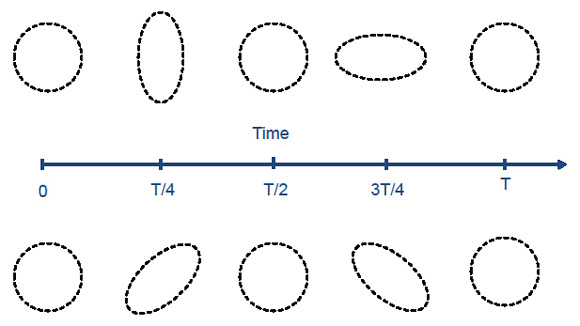
\includegraphics[scale=0.4]{./GR/GW.jpg}
\caption{Effects of a gravitational plane wave propagating along the axis $z$ on a ring of particles located in the plane $xy$, depending on the wave polarization.}
\end{figure}
\noindent
Consider the geodesic equation of a test particle in the gravitational field of a gravitational wave in the TT gauge. Since to leading order in perturbation we have $\Gamma^i_{00} = 0$, a particle initially at rest will remain at rest.
Of course, this does not mean that nothing happens , but rather that the frame of reference is co moving with the test particle. To see if anything happens , we should look at the relative motion of two neighbouring particles, which can be done using the geodesic deviation equation. The relative acceleration is given by
\[\nabla_{\bm{u}} \nabla_{\bm{u}} \bm{n} = -R(\bm{n},\bm{u}) \bm{u}.\]
To leading order in $v$, we have $u^{\mu} = (1,0)$ and $n^{\mu} = (0,n^i)$, $R{i00j} = \frac{1}{2}\ddot{h}_{ij}^{\mathrm{TT}}$. Thus that
\[\frac{d^2n^i}{dt^2} = \frac{1}{2} \ddot{h}_{ij} ^{\mathrm{TT}} n^j.\]
For $+$ modes, we have
\[\frac{d^2n^x}{dt^2} = - \frac{1}{2}\omega^2 C_{+}n^x e^{-i\omega(t-z)}, \quad \frac{d^2n^y}{dt^2} = \frac{1}{2}\omega^2 C_{+}n^y e^{-i\omega(t-z)}.\]
For $\times$ modes, we have
\[\frac{d^2n^x}{dt^2} = - \frac{1}{2}\omega^2 C_{\times}n^y e^{-i\omega(t-z)}, \quad \frac{d^2n^y}{dt^2} = - \frac{1}{2}\omega^2 C_{\times}n^x e^{-i\omega(t-z)}.\]

\section{Production of gravitational wave}
Define the Fourier transform of metric perturbation, by
\[\widetilde{\bar{h}}_{\mu\nu}(\omega, \bm{x}) \equiv \int dt e^{i\omega t} \bar{h}_{\mu\nu}(t,x).\]
In Lorentz gauge, we have
\[\widetilde{\bar{h}}_{\mu\nu}(\omega, \bm{x}) = \int d^3x' e^{i\omega R} \frac{\widetilde{T}_{\mu\nu}(\omega,\bm{x}')}{r},\]
where $r = |\bm{x} - \bm{x}'|$.
We now make the approximations that our source is isolated, far away, and slowly moving. This leaves us with
\[\widetilde{\bar{h}}_{\mu\nu}(\omega, \bm{x}) = \frac{4e^{i\omega r}}{r} \int d^3x' \tilde{T}_{\mu\nu}(\omega, \bm{x}').\]
The Lorenz gauge condition $\partial_{\mu}\bar{h}^{\mu\nu}(t,\bm{x}) = 0$ in Fourier space implies $i\omega \widetilde{\bar{h}}^{0\nu} = \partial_{i} \widetilde{\bar{h}}^{i\nu}$. 
We therefore only need to concern ourselves with the spacelike components of $\widetilde{\bar{h}}$.
We therefore want to take the integral of the spacelike components $\widetilde{T}^{\mu\nu}$. After some simplification, we can get
\[\int d^3y \widetilde{T}^{ij}(\omega,\bm{y}) = - \frac{\omega^2}{2} \int  d^3y \, y^i y^j \widetilde{T}^{00}.\]
It is conventional to define the quadrupole moment tensor of the energy density of the source,
\[I^{ij} \equiv \int d^3y \, T^{00} y^i y^j.\]
Transform back to $t$ and we can obtain the quadrupole formula,
\[\bar{h}_{ij}(t,\bm{x}) = \frac{2}{r} \frac{d^2 I_{ij}}{dt^2}(t-r).\]
One case of special interest is the gravitational radiation emitted by a binary star. 
For simplicity let us consider two stars of mass $M$ in a circular orbit in the $x-y$ plane, at distance $R$ from their common center of mass. 
We will treat the motion of the stars in the Newtonian approximation. The angular frequency of the orbit is $\Omega = (M/4R^3)^{1/2}$. 
The corresponding energy density is
\[T^{00}(t,\bm{x}) = M\delta(\bm{x}) [\delta(x-R\cos\Omega t)\delta(y-R\sin\Omega) + \delta(x+R\cos\Omega t)\delta(y+R\sin\Omega)].\]
The quadrupole moment in $x-y$ plane if the system is
\[I = MR^2 \begin{pmatrix}
1 + \cos 2\Omega t & \sin 2\Omega t \\
\sin 2\Omega t & 1 - \cos 2\Omega t
\end{pmatrix}. \]
Thus the spacelike metric perturbation in $x-y$ plane is
\[\bar{h} = \frac{8M\Omega^2R^2}{r} \begin{pmatrix}
- \cos 2\Omega (t-r) & -\sin 2\Omega (t-r) \\
-\sin 2\Omega (t-r) & + \cos 2\Omega (t-r)
\end{pmatrix}. \]

\section{External field of a gravitating source}
Consider an isolated system with gravity so weak that in calculating its structure and motion one can completely ignore self-gravitational effects. We can work out the weak gravitational field,
\[\bar{\bar{h}}_{\mu\nu}(t,\bm{x}) \equiv h_{\mu\nu}(t,\bm{x}) = \int \frac{4\bar{T}_{\mu\nu}(t-R,\bm{x}')}{R} d^3x',\]
produced by such a system. Restrict attention to the spacetime region far outside the system, and expand $h_{\mu\nu}$ in powers of $\bm{x}' / {r}$, we can get
\begin{eqnarray}
ds^2 &=& -\left[1-\frac{2M}{r} + O({1}/{r^3}) \right]dt^2 - \left[4\epsilon_{jkl}S^k \frac{x^l}{r^3} + O({1}/{r^3})  \right] dtdx^i  \nonumber \\
&+& \left[(1+\frac{2M}{r})\delta_{jk} + \mbox{ gravitational radiation terms that die out as } O(1/r) \right]dx^j dx^k , \nonumber
\end{eqnarray}
where
\[M \equiv \int T^{00}d^3x , \quad S_k \equiv \int \epsilon_{klm}x^l T^{m0} d^3x .\]
It is plausible to say the mass of the system is $M$ and the angular momentum $\bm{S}$. With an appropriate choice of gauge, $g_{00}$ far from any weak source are time-independent and are determined uniquely by the source's mass $M$; $g_{0j}$ is time-independent and is fixed by the source's intrinsic angular momentum $S^j$; but $g_{jk}$ has time-dependent terms (gravitational waves) of $O(1/r)$.
\\ \\
The values of a system's mass and angular momentum can be measured by probing the imprint they leave in its external gravitational field. 
Of all tools one might use to probe, the simplest is a test particle in a gravitationally bound orbit. 
If the particle is sufficiently far from the source, its motion is affected hardly at all by the source's angular momentum or by the gravitational waves; only the spherical, Newtonian part of the gravitational field has a significant influence. 
Hence, the particle moves in an elliptical Keplerian orbit. To determine the source's mass $M$, one need only apply Kepler's third law
\[M = \left( \frac{2\pi}{\mbox{orbital period}} \right)^2 \left(\mbox{ Semi-major axis of ellipse } \right)^3.\]
Angular momentum can be probed by a gyroscope.
Place a gyroscope at rest in the source's gravitational field.
By a force applied to its center of mass, prevent it from falling. 
As time passes, the $g_{0j}$ term in the metric will force the gyroscope to precess relative to the basis vectors $\frac{\partial}{\partial x^j}$; and since these basis vectors are ``tied'' to the coordinate system, which
in turn is tied to the Lorentz frames at infinity, which in turn are tied to the ``fixed stars'' , the precession is relative to the ``fixed stars.'' 
The angular velocity of precession is
\[\bm{\Omega} = \frac{1}{r^3} \left[ -\bm{S} + \frac{3(\bm{S}\cdot \bm{x})\bm{x}}{r^3} \right] .\]
One sometimes says that the source's rotation ``drags the inertial frames near the source,'' thereby forcing the gyroscope to precess.
\\ \\
Consider an isolated, gravitating system inside which spacetime may or may not be highly curved. We restrict attention to the weak gravitational field far from the source, and analyze it using linearized theory in vacuum.
Expand $h_{\mu\nu}$ in multipole moments and powers of $1/r$; and adjust the gauge, the Lorentz frame, and the origin of coordinates to simplify the resulting metric.
We have
\begin{eqnarray}
ds^2 &=& -\left[1-\frac{2M}{r} + \frac{2M^2}{r^2} + O({1}/{r^3}) \right]dt^2 - \left[4\epsilon_{jkl}S^k \frac{x^l}{r^3} + O({1}/{r^3})  \right] dtdx^i  \nonumber \\
&+& \left[(1+\frac{2M}{r} + \frac{3M^2}{2r^2})\delta_{jk} + \mbox{ gravitational radiation terms that die out as } O({1}/{r}) ) \right]dx^j dx^k. \nonumber
\end{eqnarray}
However, $M$ and $\bm{S}$ is not a simple integration of $T^{00}$ and $\epsilon_{klm} x^l T^{0m}$ of the system as in the case of weakly gravitating sources.
However, since this integration is impossible to measure in practice. We always determine the mass of the star by studying the orbits of planets in its external gravitational field. Therefore, one defines the ``total mass-energy'' $M$ of the sun or other body to be the constant that appears in the line element for its distant external spacetime geometry. Similarly, one defines the body's intrinsic angular momentum as the constant 3-vector $\bm{S}$ appearing in its line element.

\section{Conservation laws for 4-momentum and angular momentum}
Recall in the weak field limit, the Einstein equation can be written as
\[H^{\mu\alpha\nu\beta}_{\phantom{****},\alpha
\beta} = 16\pi T^{\mu\nu}.\]
Thus we have
\[T^{\mu\nu}_{\phantom{**},\nu} = \frac{1}{16\pi}H^{\mu\alpha\nu\beta}_{\phantom{****},\alpha\beta\nu} = 0.\]
The source's total 4-momentum can be defined as
\[P^{\mu} \equiv \int T^{\mu 0}d^3x = \frac{1}{16\pi} \oint_{S} H^{\mu\alpha 0 j}_{\phantom{****},\alpha} d^2 S_j .\]
Particularly, we have
\[P^0 = \frac{1}{16\pi} \oint_{S} (g_{jk,k} - g_{kk,j})d^2S_{j} .\]
The angular momentum of the source can be defined as
\[J^{\mu\nu} \equiv \int (x^{\mu} T^{0\nu} - x^{\nu} T^{0\mu}) d^3x  = \frac{1}{16\pi} \oint_S (x^{\mu}H^{\nu\alpha 0 j}_{\phantom{****},\alpha} - x^{\nu}H^{\mu\alpha 0 j}_{\phantom{****},\alpha} + H^{\mu j 0 \nu} - H^{\nu j 0 \nu}) d^2 S_j .\]
\begin{note}
To evaluate the flux integrals (by contrast with the volume
integrals), one need utilize only the gravitational field far outside the source. Since that gravitational field has the same form in full general relativity for strong sources as in linearized theory for weak sources, the flux integrals can be used to figure out $P^{\mu}$ and $J^{\mu\nu}$ for any isolated source whatsoever, weak or strong. Thus we will use the flux integrals as the definition.
\end{note}

\noindent
Knowing $P^{\mu}$ and $J^{\mu\nu}$, one can figure out the source's total mass-energy $M$ intrinsic angular momentum $S_{rho}$ by
\[M = (-P^{\mu}P_{\mu})^{-1/2};\]
\[Y^{\mu} = -J^{\mu\nu}P_{\nu}/M^2;\]
\[S_{\rho} = \frac{1}{2}\epsilon_{\mu\nu\sigma\rho}(J^{\mu\nu} - Y^{\mu}P^{\nu} + Y^{\nu}P^{\mu})P^{\sigma}/M.\]
Note especially that the integrands of the flux integrals  are not gauge-invariant. In any local inertial frame at an event they vanish. 
However, the total integrals $P^{\mu}$ and $J^{\mu\nu}$ are. 
They have meaning and significance independent of any coordinate system and gauge. They are tensors in the asymptotically flat region surrounding the source.
\\ \\
In full general relativity, though $|h_{\mu\nu}| \ll 1$ breaks down, we can still define formally
\[-H^{\mu\alpha\nu\beta} \equiv \overline{h}^{\mu\nu}\eta^{\alpha\beta} + \overline{h}^{\alpha\beta}\eta^{\mu\nu} - \overline{h}^{\alpha\nu}\eta^{\mu\beta} - \overline{h}^{\mu\beta}\eta^{\alpha\nu} , \quad h_{\mu\nu} \equiv g_{\mu\nu} - \eta_{\mu\nu}.\]
And we define the effective energy-momentum pseudotensor by
\[H^{\mu\alpha\nu\beta}_{\phantom{****},\alpha
\beta} = 16\pi T^{\mu\nu}_{\mathrm{eff}}.\]
Therefore, we have
\[T^{\mu\nu}_{\mathrm{eff},\nu} = 0.\]
\[P^{\mu} = \frac{1}{16\pi} \int d^3x T^{\mu0}_{\mathrm{eff}};\]
\[J^{\mu\nu} = \int (x^{\mu} T^{0\nu}_{\mathrm{eff}} - x^{\nu} T^{0\mu}_{\mathrm{eff}}) d^3x.\]
for both strong or weak source.
Define gravitation energy-momentum pseudotensor as
\[16\pi t^{\mu\nu} \equiv H^{\mu\alpha\nu\beta}_{\phantom{****},\alpha
\beta} - 2G^{\mu\nu},\]
so we have $T^{\mu\nu}_{\mathrm{eff}} = T^{\mu\nu} + t^{\mu\nu}$. 
All the quantities $H^{\alpha\mu\nu\beta}$, $t^{\mu\nu}$ and $T^{\mu\nu}_{\mathrm{eff}}$ depend for their definition and existence on the choice of coordinates.
There is, nevertheless, adequate invariance under general coordinate transformations to give the values $P^{\mu}$ and $J^{\mu\nu}$ of the volume integrals geometric, coordinate-free significance in the asymptotically flat region far outside the source.
Although this invariance is hard to see in the volume integrals themselves, it is clear from the surface-integral forms that no coordinate transformation which changes the coordinates only inside some spatially bounded region can influence the values of the integrals. 
For coordinate changes in the distant, asymptotically
flat regions, linearized theory guarantees that under Lorentz transformations the integrals for $P^{\mu}$ and $J^{\mu\nu}$ will transform like special relativistic tensors, and that under infinitesimal coordinate transformations (gauge changes) they will be invariant.
\\ \\
It is clear that any quantities $H^{\alpha\mu\nu\beta}_{\mathrm{new}}$  which agree with the original $H^{\alpha\mu\nu\beta}$ in the asymptotic weak-field region will give the same values as $H^{\alpha\mu\nu\beta}$ does for the $P^{\mu}$ and $J^{\mu\nu}$ surface integrals. One especially convenient
choice is Landau-Lifshitz pseudotensor. The details can be found in section 96 of \emph{The Classical Theory of Fields (L.D.Landau \& E.M.Lifshitz)}
For a system of gravitating bodies, we have
\[\frac{dP^{\mu}}{dt} = -\oint T^{\mu j}_{\mathrm{eff}}d^2S_j ;\]
\[\frac{dJ^{\mu\nu}}{dt} = -\oint(x^{\mu}T^{\nu j}_{\mathrm{eff}} - x^{\nu}T^{\mu j}_{\mathrm{eff}}) d^2 S_j.\]
The flux is integrated over the surface in asymptomatic flat region. Although the pseudotensor $t^{\mu\nu}$ in the interbody region and outside the system, contributes negligibly to the total 4-momentum and angular momentum, its contribution via gravitational waves to the time derivatives can be important when added up over astronomical periods of time. Thus, one must not ignore it in the flux integrals.
\\ \\
There are some limitations on our interpretation of $t_{\mu\nu}$ as an energy-momentum tensor. 
It is not invariant  under gauge transformations. 
One way of circumventing this difficulty is to average the energy-momentum tensor over several wavelengths, an operation we denote by angle brackets $\langle \cdots \rangle$.
Since any terms that are derivatives (as opposed to products of derivatives) will average to zero, we are therefore empowered to integrate by parts under the averaging brackets,
\[\langle A(\partial_{\mu} B) \rangle = - \langle (\partial_{\mu} A)B \rangle.\]
After a lot of messy intermediate steps, we will arrive at
\[t_{\mu\mu} = \frac{1}{32\pi} \left\langle (\partial_{\mu}h_{\rho\sigma})(\partial_{\nu}h^{\rho\sigma}) - \frac{1}{2} \partial_{\mu} h \partial_{\nu} h - (\partial_{\rho}h^{\rho\sigma})(\partial_{\mu}h_{\nu\sigma}) - (\partial_{\rho}h^{\rho\sigma})(\partial_{\nu}h_{\mu\sigma})\right\rangle + O(h^3).\]
Since we only care about $t_{\mu\nu}$ in vacuum far from the source, we can adopt TT gauge and neglect higher order terms. 
For a ``monochromatic'' plane gravitational wave $h^{\rm TT}_{\mu\nu} = C_{\mu\nu} \sin(k^{\sigma}x_{\sigma})$, the energy- momentum tensor is
\[t_{\mu\nu} = \frac{1}{64\pi} k_{\mu}k_{\nu} {\rm Tr}(C^2).\]
It the wave is propagating along $z$ direction, we have
\[t^{\mu\nu} = \frac{\pi}{8G} f^2(C_{+}^2 + C_{\times}^2) \begin{pmatrix}
1 & 0 & 0 & 1 \\
0 & 0 & 0 & 0 \\
0 & 0 & 0 & 0 \\
1 & 0 & 0 & 1 
\end{pmatrix}, \]
where $f = \omega / 2\pi$ is the frequency of gravitational wave.
We now can use our formula for the gravitational-wave energy-momentum tensor to calculate the rate of energy loss from a system emitting gravitational radiation
according to the quadrupole formula. We omit the derivation here and write down the final expression directly,
\[P = -\frac{1}{5}\left\langle \frac{d^3 J_{ij}}{dt^3} \frac{d^3 J^{ij}}{dt^3}  \right\rangle,  \]
where $J_{ij} \equiv I_{ij} - 1/3 \delta_{ij} {\rm Tr}I$, called reduced quadrupole moment. The power of gravitational wave generated by binary stars is
\[P = \frac{2}{5} \frac{M^5}{R^5}.\]

\chapter{Black Holes}
\section{Schwarzschild black hole}
\subsection{Schwarzschild metric}
In spherical coordinates $\{t,r,\theta,\phi\}$, the metric is given by
\[ds^2 = -\left(1 - \frac{2M}{r} \right)dt^2 + \left(1 - \frac{2M}{r} \right)^{-1}dr^2 + r^2 d\Omega^2,\]
where $d\Omega^2$ is the metric on a unit two-sphere,
\[d\Omega^2 = d\theta^2 + \sin^2\theta d\phi^2.\]

\begin{newthem}[Birkhoff's theorem]
Schwarzschild metric is the unique vacuum solution with spherical symmetry.
\end{newthem}
\noindent
The proof can be found in section 5.2 of \emph{Spacetime and Geometry (Sean Carroll)}. 
Any spherically symmetric vacuum metric possesses a timelike Killing vector. A metric that possesses a Killing vector that is timelike near infinity is called stationary. A metric is called static if it possesses a timelike Killing vector that is orthogonal to a family of hypersurfaces. 
An alternative definition of ``static'' is stationary, and invariant under time reversal. We should think of stationary as meaning ``doing exactly the same thing at every time,'' while static means ``not doing anything at all.''
\\ \\
The Schwarzschild metric coefficients become infinite at $r = 0$ and $r = 2M$. 
The metric coefficients are coordinate-dependent quantities, it is certainly possible to have a coordinate singularity that results from a breakdown of a specific coordinate system rather than the underlying manifold. 
Direct calculation reveals that
\[R^{\mu\nu\rho\sigma}R_{\mu\nu\rho\sigma} = \frac{48M^2}{r^6}.\]
This is enough to convince us that $r = 0$ represents an honest singularity.
\\ \\
As for $r = 2M$, the Schwarzschild radius. We can check that none of the curvature invariants blows up there. We therefore begin to think that it is actually not singular, and we have simply chosen a bad coordinate system. The surface $r = 2M$ is very well-behaved in the Schwarzschild metric -- it demarcates the event horizon of a black hole.

\subsection{Geodesics of Schwarzschild spacetime}
There are four Killing vectors in Schwarzschild Space-time: three for the spherical symmetry, and one for time translations.
Each of these will lead to a constant of the motion for a free particle.
If $K_{\mu}$ is a Killing vector, we know that
\[K_{\mu} \frac{dx^{\mu}}{d\lambda}.\]
Here, we choose the affine parameter $\lambda$ of geodesics to make $dx^{\mu}/d\lambda$ four velocity for massive particles and four momentum for massless particles. Thus the quantity
\[\epsilon = -g_{\mu\nu} \frac{dx^{\mu}}{d\lambda} \frac{dx^{\mu}}{d\lambda}\]
is constant along the path. For massive particles $\epsilon = 1$ while for massless particles, $\epsilon = 0$.
\\ \\
We can think of the angular momentum as a three-vector with a magnitude (one component) and direction (two components). 
Conservation of the direction of angular momentum means that the particle will move in a plane. We can choose this to be the equatorial plane of our coordinate system. Thus, the two Killing vectors that lead to conservation of the direction of angular momentum imply that, for a single particle, we can choose
\[\theta = \frac{\pi}{2}.\]
The two remaining Killing vectors correspond to energy and the magnitude of angular momentum. The energy arises from the timelike Killing vector
\[K^{\mu} = (\partial_t)^{\mu} = (1,0,0,0), \; K_{\mu} = (\frac{2M}{r}-1, 0,0,0)\]
The Killing vector whose conserved quantity is the magnitude of the angular momentum is
\[R^{\mu} = (\partial_{\phi})^{\mu} = (0,0,0,1), \; R_{\mu} = (0,0,0,r^2\sin^2\theta) \]
The two conserved quantities are
\[E = -K_{\mu} \frac{dx^{\mu}}{d\lambda} = \left( 1- \frac{2M}{r}\right) \frac{dt}{d\lambda}, \; L = R_{\mu} \frac{dx^{\mu}}{d\lambda} = r^2\frac{d\phi}{d\lambda}\]
For massless particles, these can be thought of as the conserved energy and angular momentum, while for massive particles they are the conserved energy and angular momentum per unit mass of the particle.
\\ \\
After some algebra manipulations, we can get a single equation for $r(\lambda)$,
\[\frac{1}{2} \left( \frac{dr}{d\lambda} \right)^2 + V(r) = \mathcal{E},\]
where
\[V(r) = \frac{1}{2}\epsilon - \epsilon \frac{M}{r} + \frac{L^2}{2r^2} - \frac{ML^2}{r^3}\]
and
\[\mathcal{E} = \frac{1}{2}E^2.\]

\begin{figure}
\centering
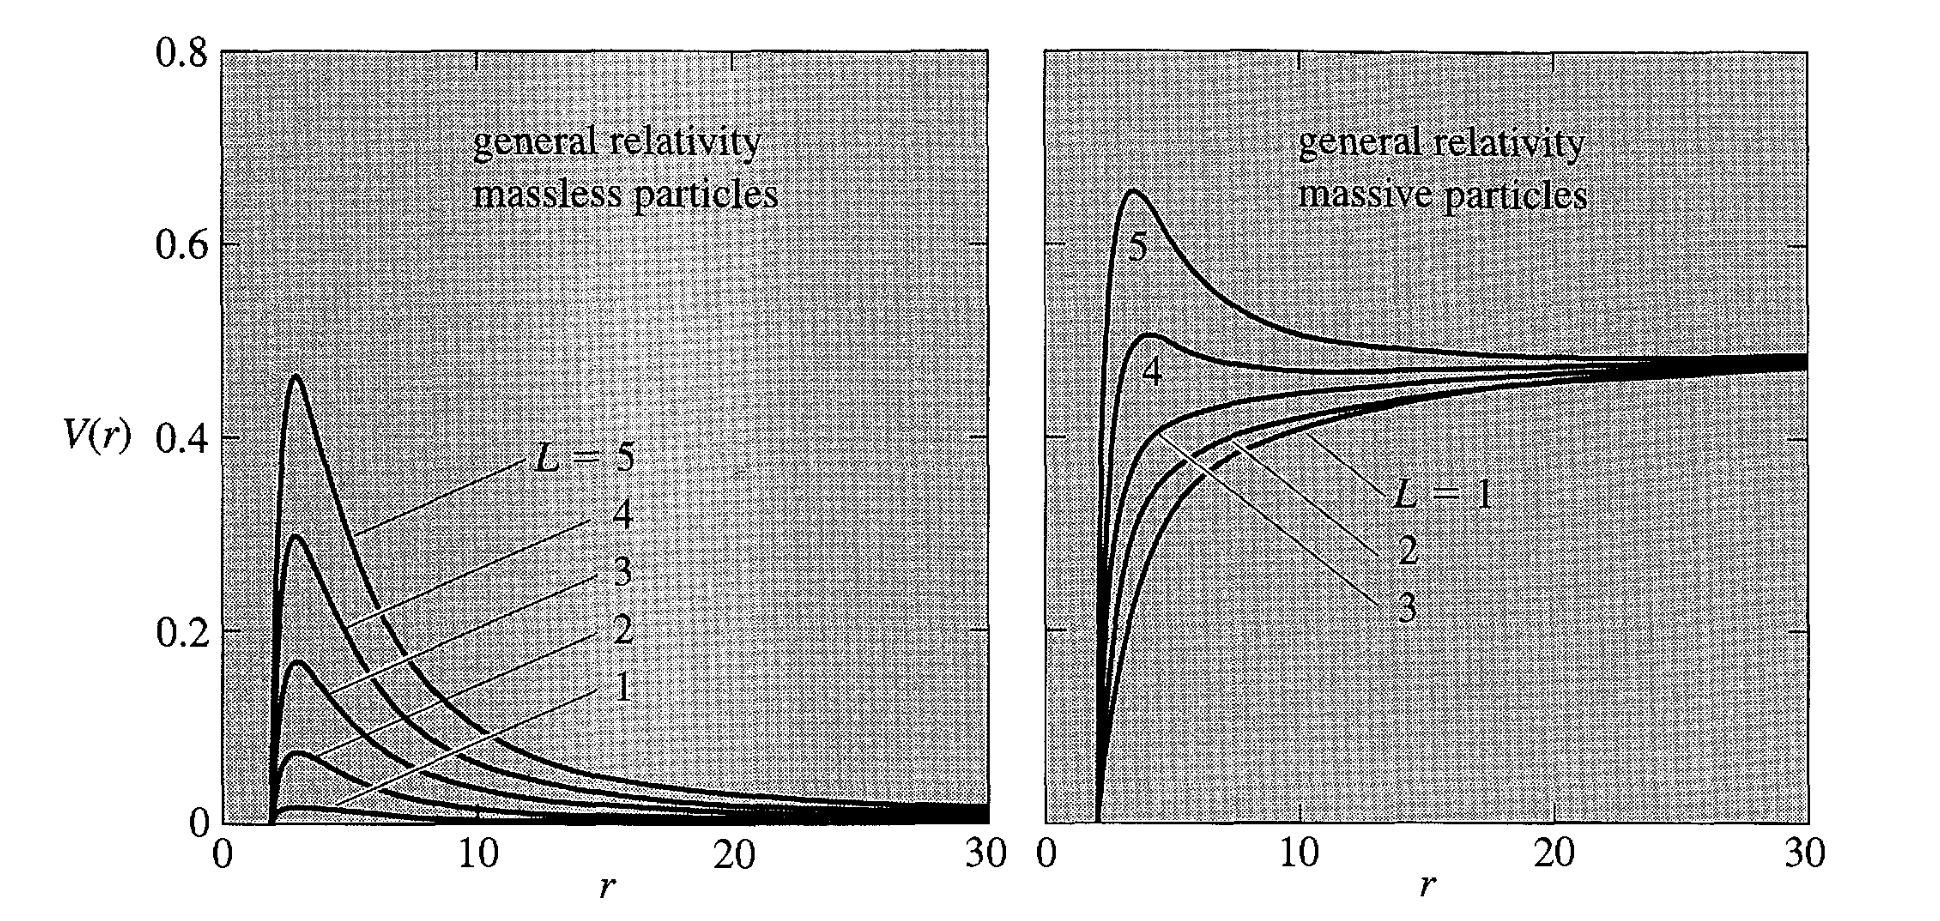
\includegraphics[scale=0.2]{GR/EP1.png}
\caption{Effective potentials in general relativity. We have chosen $M = 1$. In GR there is an innermost circular orbit greater than or equal to $3M$, and any orbit that falls inside this radius continues to $r = 0$ (for particles on geodesies).}
\end{figure}

\noindent
In general relativity, at $r = 2M$ the potential is always zero; inside this radius is the black hole.
For massless particles there is always a barrier (except for $L = 0$, for which the potential vanishes identically), but a sufficiently energetic photon will  nevertheless go over the barrier and be dragged inexorably down to the center. At the top of the barrier are unstable circular orbits $r_{\rm c} = 3M$.
\\ \\
For massive particles, the circular orbits are at
\[r_{\rm c} = \frac{L^2 \pm \sqrt{L^4-12M^2L^2}}{2M}.\]
For large $L$ there will be two circular orbits, one stable and one unstable. In the $L \to \infty$ limit their radii are given by $r_{\rm c} = \left(L^2/M, 3GM \right)$.
In this limit the stable circular orbit becomes farther away, while the unstable one approaches $3M$, behaviour that parallels the massless case. As we decrease $L$,
the two circular orbits come closer together; they coincide when $L = \sqrt{12}M$ for which $r_{\rm c} = 6M$. We have therefore found that the Schwarzschild solution possesses stable circular orbits for $r > 6M$ and unstable circular orbits for $3M < r < 6M$. 
It's important to remember that these are only the geodesies; there is nothing to stop an accelerating particle from dipping below $r = 3M$ and emerging, as long as it stays beyond $r = 2M$.
\\ \\
As for a general non-circular orbit, we have the equation for orbit
\[\left(\frac{dr}{d\phi}\right)^2 + \frac{1}{L^2}r^4 - \frac{2M}{L^2}r^3 + r^2 - 2Mr = \frac{2E}{L^2}r^4. \] 
Define $x \equiv L^2/Mr$, we can get
\[\left(\frac{dx}{d\phi}\right)^2 + \frac{L^2}{M^2} - 2x + x^2 - \frac{2M^2}{L^2}x^3 = \frac{2EL^2}{M^2}. \]
Then we differentiate equation above with respect to $\phi$ to get
\[\frac{d^2x}{d\phi^2} - 1 + x = \frac{3M^2}{L^2}x^2.\]
In a Newtonian calculation, the last term would be absent, and we could solve for $x$ exactly; here, we suppose the orbit is far from horizon and treat it as a perturbation.
We expand $x$ into a Newtonian solution plus a small deviation, $x = x_0 + x_1$. The solution for the zeroth-order equation can be written as
\[x_0 = 1 + e\cos\phi.\]
Thus the first-order equation will be
\[\frac{d^2x_1}{d\phi^2} + x_1 = \frac{3M^2}{L^2}(1+e\cos\phi)^2.\]
After some approximation, we can get
\[x = 1 + e\cos((1-\alpha)\phi),\]
where $\alpha = 3M^2/L^2$. During each orbit, perihelion 
advances by an angle
\[\Delta \phi = 2\pi \alpha = \frac{6\pi M^2}{L^2}.\]
An ordinary ellipse satisfies
\[r = \frac{(1-e^2)a}{1+e\cos\phi},\]
where $a$ is the semi-major axis. Comparing to our zeroth-order solution and the definition of $x$, we see that
\[L^2 \approx M(1-e^2)a.\]
Finally, we have
\[\Delta \phi = \frac{6\pi M}{(1-e^2)a}.\]

\begin{figure}[!htb]
\centering
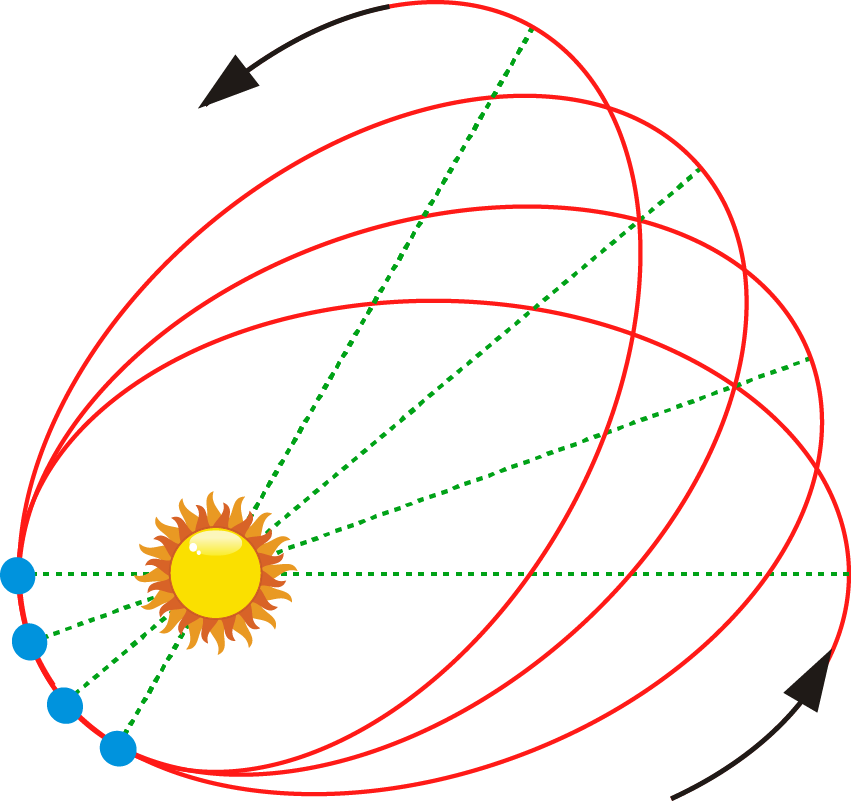
\includegraphics[scale=0.35]{GR/perihelion.png}
\caption{Perihelion of Mercury.}
\end{figure}

\subsection{Penrose diagram and event horizon}
In theoretical physics, a Penrose diagram is a two-dimensional diagram capturing the causal relations between different points in spacetime. 
It is an extension of a Minkowski diagram where the vertical dimension represents time, and the horizontal dimension represents space, and slanted lines at an angle of $45^{\circ}$ correspond to light rays. 
The biggest difference is that locally, the metric on a Penrose diagram is conformally equivalent to the actual metric in spacetime. 
The conformal factor is chosen such that the entire infinite spacetime is transformed into a Penrose diagram of finite size. 
For spherically symmetric spacetime, every point in the diagram corresponds to a $2$-sphere.
\\ \\
The metric of Minkowski space-time is 
\[ds^2 = -dt^2 + dr^2 + r^2 d\Omega^2.\]
Introduce the new coordinates $T$ and $R$ by 
\[t + r = \tan \frac{T+R}{2} ,\quad t - r = \tan \frac{T-R}{2}.\]
The metric can be written as
\[ds^2 = \frac{-dT^2+dR^2}{4\cos^2\frac{T+R}{2} \cos^2 \frac{T-R}{2}} + r^2(T,R) d\Omega^2.\]
The range of the new coordinates are $0 \leq R < \pi$ and  $|T| + R < \pi$.

\begin{figure}[!htb]
\centering
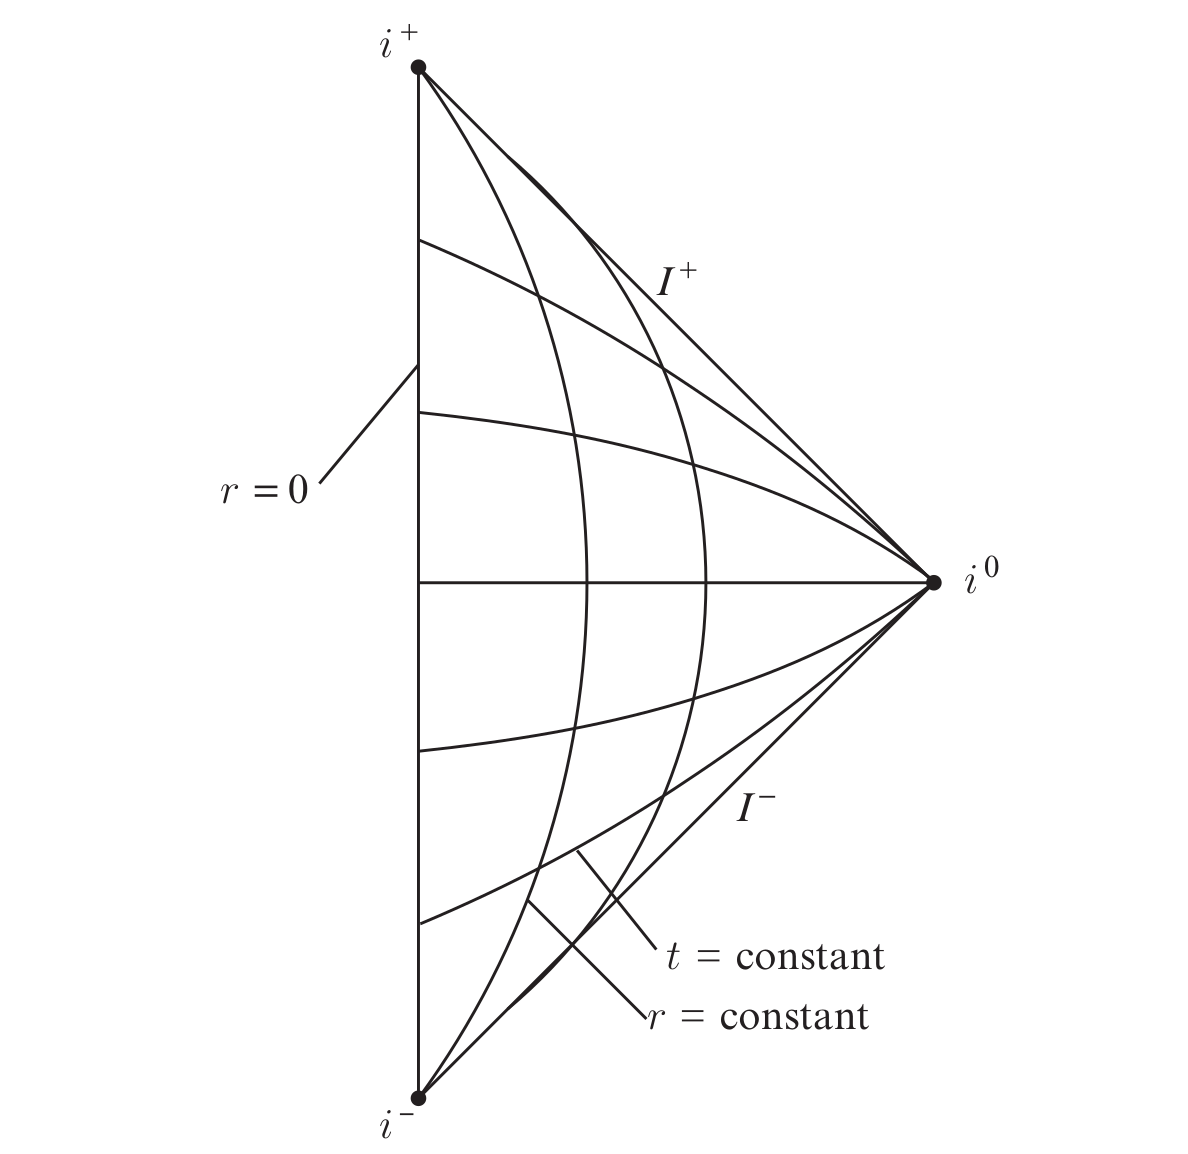
\includegraphics[scale=0.15]{GR/Penrose1.png}
\caption{Penrose diagram of Minkowski spacetime}
\end{figure}

\noindent
It is obvious that light cones are still 45 degree lines in this Penrose diagram. 
What is more, points and regions located at infinite distances in the original coordinates have now been brought to a finite distance. 
The figure indicates a set of different kinds of ``infinity'' that is useful in the discussion of physical phenomena. The following list gives the definition of each of these.
\begin{eqnarray}
i^{+} &=& \mbox{ future timelike infinity } (T = \pi, R = 0) \nonumber \\
i^{0} &=& \mbox{ spatial infinity } (T = 0, R = \pi) \nonumber \\
i^{-} &=& \mbox{ past timelike infinity } (T = -\pi, R = 0) \nonumber \\
I^{+} &=& \mbox{ future null infinity } (T = \pi - R, 0 < R < \pi) \nonumber \\
I^{-} &=& \mbox{ past null infinity } (T = -\pi + R, 0 < R < \pi) \nonumber
\end{eqnarray}
\\
Black holes are characterized by the fact that you can enter them, but never exit. 
Thus, their most important feature is actually not the singularity at the center, but the event horizon at the boundary. 
An event horizon is a hypersurface separating those spacetime points that are connected to infinity by a timelike path from those that are not. 
In general relativity, the global structure of spacetime can take many different forms, with correspondingly  different notions of infinity. 
But to think about black holes in the real universe, we use infinity as a proxy for ``well outside the black hole,'' and imagine that spacetime sufficiently far away from the hole can be approximated by Minkowski space.
\begin{figure}[!htb]
\centering
\includegraphics[scale=0.25]{GR/Penrose2.eps}
\caption{Penrose diagram of event horizon}
\end{figure}

\noindent
From Penrose diagram, the future event horizon is the surface beyond which timelike curves cannot escape to infinity. 
The causal past $J^{-}$ of a region is the set of all points we can reach from that region by moving along past-directed timelike paths, the event horizon can be
equivalently defined as the boundary of $J^{-}(I^+)$, the causal past of future null infinity. Analogous definitions hold for the past horizon. From the definition, it is clear that the event horizon is a null hypersurface.

\subsection{The maximally extended Schwarzschild solution}
Let us consider radial null curves, those for which $\theta$ and $\phi$ are constant and $ds^2 = 0$. We can get
\[\frac{dt}{dr} = \pm \left(1 -\frac{2M}{r} \right)^{-1}\]
For large $r$ the slope is $\pm$, as it would be in flat space, while as we approach $r = 2M$ we get $dt / dr = \pm \infty$, and the light cones ``close up''. 
Thus a light ray that approaches $r = 2M$ never seems to
get there, at least in this coordinate system; instead it seems to asymptote to this radius.

\begin{figure}[!htb]
\centering
\includegraphics[scale=0.3]{GR/BH1.eps}
\caption{In Schwarzschild coordinates, light cones appear to close up as we approach $r = 2M$.}
\end{figure}

\noindent
If we stayed outside while an intrepid observational general relativist dove into the black hole, sending back
signals all the time, we would simply see the signals reach us more and more slowly.

\begin{figure}[!htb]
\centering
\includegraphics[scale=0.3]{GR/BH2.eps}
\caption{A beacon falling freely into a black hole emits signals at intervals of constant proper time. An observer at fixed $r$ receives the signals at successively longer
time intervals.}
\end{figure}

\noindent
The fact that we never see the infalling observer reach $r = 2M$ is a meaningful statement, but the fact that their trajectory in the $t-r$ plane never reaches there is not. 
It is highly dependent on our coordinate system, and we would like to ask a more coordinate-independent question (such as, ``Does the observer reach this radius in a finite amount of their proper time?''). 
The best way to do this is to change coordinates to a system that is better behaved at $r = 2M$. We omit the intermediate steps of coordinate transformation and move to Kruskal coordinates directly. The new coordinates is given by
\[T = \left( \frac{r}{2M} -1 \right)^{1/2} e^{r/4M}\sinh \left( \frac{t}{4M}\right), \quad R = \left( \frac{r}{2M} -1 \right)^{1/2} e^{r/4M}\cosh\left( \frac{t}{4M}\right).\]
The metric becomes
\[ds^2 = \frac{32M^3}{r}e^{-r/2M}(-dT^2+dR^2) + r^2 d\Omega^2.\]
We can now draw a spacetime diagram in the $T-R$ plane, known as a Kruskal diagram. This diagram represents the maximal extension of the Schwarzschild geometry; the coordinates cover what we should think of as
the entire manifold described by this solution.

\begin{figure}[!htb]
\centering
\includegraphics[scale=0.3]{GR/BH3.eps}
\caption{The Kruskal diagram -- the Schwarzschild solution in Kruskal coordinates, where all light cones are at $\pm 45^{\circ}$.}
\end{figure}

\noindent
\\
Finally, we can further transform the coordinates to bring them into a finite range and get the Penrose diagram of Schwarzschild spacetime.

\begin{figure}[!htb]
\centering
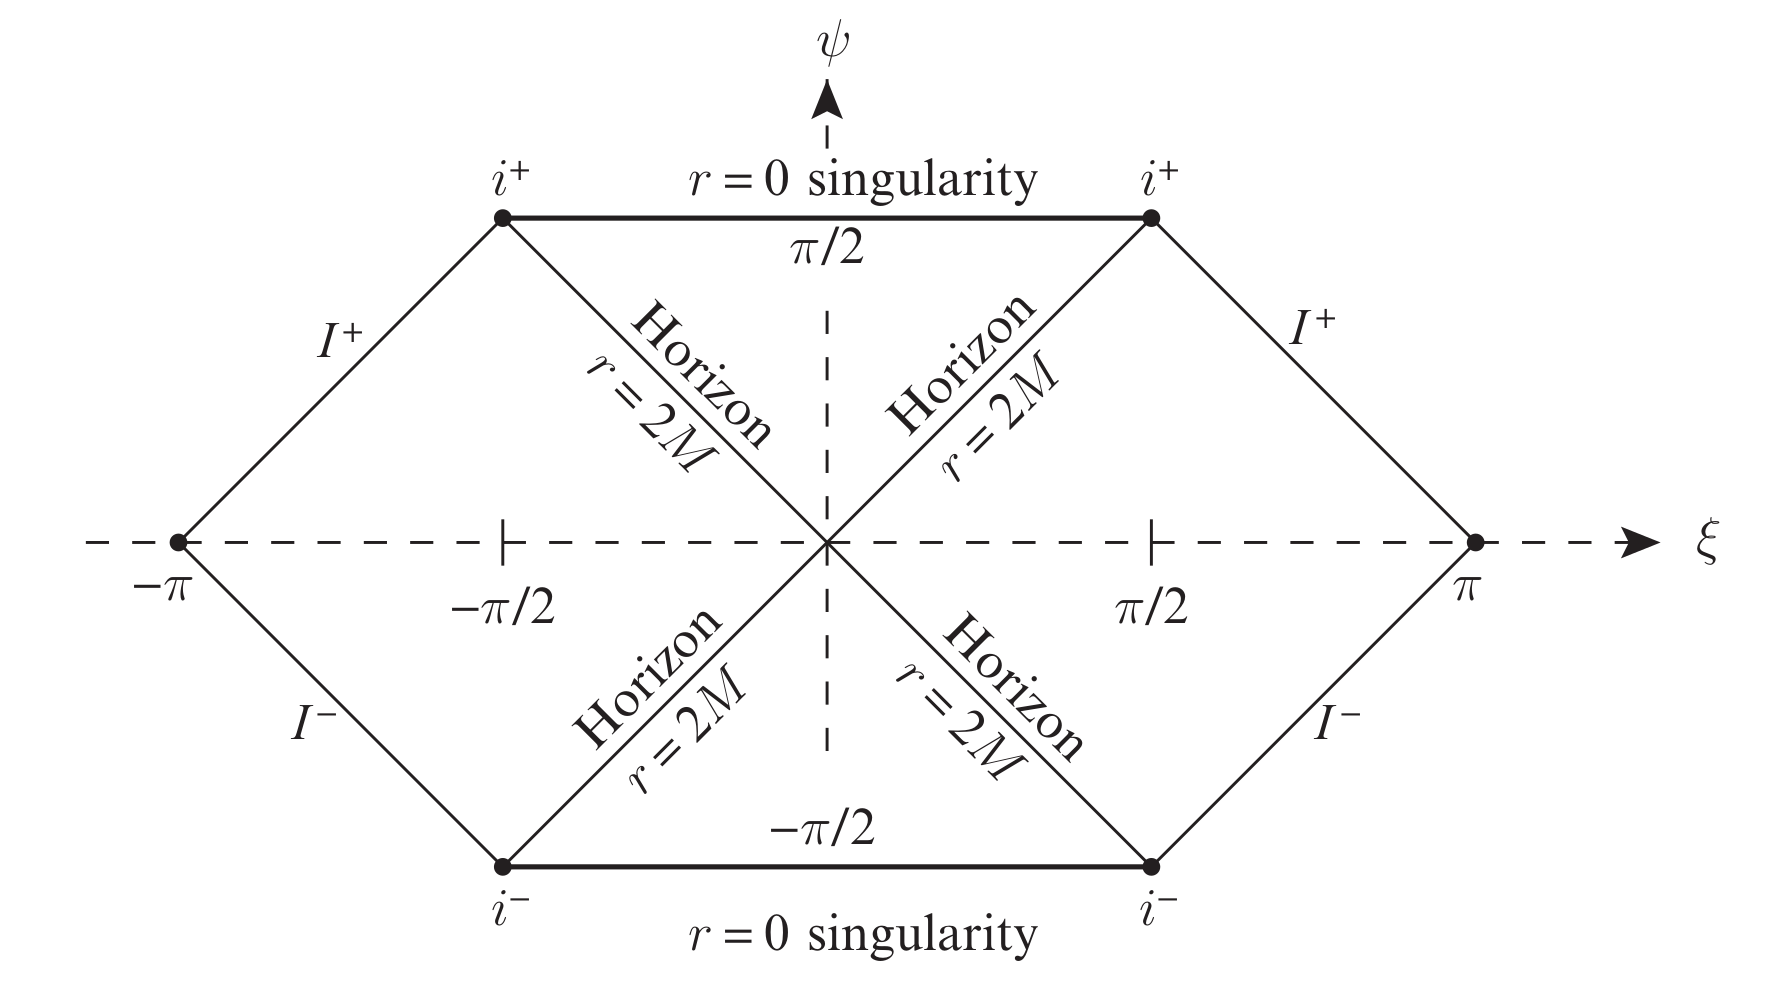
\includegraphics[scale=0.15]{GR/BH4.png}
\caption{The Penrose diagram for the Schwarzschild spacetime.}
\end{figure}

\section{Reissner-Nordstrom black hole}
The metric of Reissner-Nordstrom black hole is
\[ds^2 = -\Delta dt^2 + \Delta^{-1}dr^2 + r^2d\Omega^2,\]
where
\[\Delta = 1 - \frac{2M}{r} + \frac{Q^2}{4 \pi r^2}.\]
The EM filed is given by
\[A_{t} = -\frac{Q}{4\pi r}.\]
The RN metric has a true curvature singularity at $r = 0$, as could be checked by computing the curvature invariant scalar $R^{\mu\nu\rho\sigma}R_{\mu\nu\rho\sigma}$. 
The horizon of RN metric is given by $g^{r}{r} = 0$, i.e.
\[1 - \frac{2M}{r} + \frac{Q^2}{4 \pi r^2} = 0.\]
\\
If $M^2 > Q^2 / 4 \pi$, the metric coefficient $\Delta$ is positive at large $r$ and small $r$, and negative inside the two vanishing points $r_{\pm} = M \pm \sqrt{M^2 - Q^2 / 4 \pi}$. 
The metric has coordinate singularities at both $r_{+}$ and $r_{-}$; in both cases these could be removed by a change of coordinates as we did with Schwarzschild.
The surfaces defined by $r_{\pm}$ are both null, and they are both event horizons. 
The singularity at $r = 0$ is a timelike line, not a spacelike surface as in Schwarzschild. 
If you are an observer falling into the black hole from far away, $r_{+}$ is just like $2M$ in the Schwarzschild metric; at this radius $r$ switches from being a spacelike coordinate to a timelike coordinate, and you necessarily move in the direction of decreasing $r$. 
Witnesses outside the black hole also see the same phenomena that they would outside an uncharged hole --- the infalling observer is seen to move more and more slowly, and is increasingly redshifted.
\\ \\
But the inevitable fall from $r_{+}$ to ever-decreasing radii only lasts until you reach the null surface $r = r_{-}$, where $r$ switches back to being a spacelike 
coordinate and the motion in the direction of decreasing r can be arrested. 
You can choose either to continue on to $г = 0$, or begin to move in the direction of increasing $r$ back through the null surface at $r = r_{-}$.
Then $r$ will once again be a timelike coordinate, but with reversed orientation; you are forced to move in the
direction of increasing $r$. 
You will eventually be spit out past $r = r_{+}$ once more, which is like emerging from a white hole into the rest of the universe.
From here you can choose to go back into the black hole --- this time, a different hole than the one you entered in the first place --- and repeat the voyage as many times as you like.
\\ \\
If $M^2 = Q^2 / 4 \pi$, the extremal black holes have $\Delta = 0$ at a single radius, $r = M$. 
This represents an event horizon, but the $r$ coordinate is never timelike; it becomes null at $г = M$, but is spacelike on either side. 
The singularity at $r = 0$ is a timelike line, as in the other cases.
 Thus for this black hole you can again avoid the singularity and continue to move to the future to extra copies of the asymptotically flat region, but the singularity is always ``to the left''. 
\\ \\
If $M^2 < Q^2 / 4 \pi$, $\Delta$ is always positive and the metric is completely all the way down to $r = 0$. 
The coordinate $t$ is always timelike, and $r$ is always spacelike. But still there is the singularity at $r = 0$, which is now a timelike line. 
Since there is no event horizon, there is no obstruction to an observer traveling to the singularity and returning to report on what was observed. 
This is a naked singularity. 
A careful analysis of the geodesies reveals that the singularity is repulsive--timelike geodesies never intersect $r = 0$; instead they approach and then reverse course and move away. 
Null geodesies can reach the singularity, as can nongeodesic timelike curves.
As $r \to \infty$ the solution approaches flat spacetime, and as we have just seen the causal structure seems normal everywhere. 
The conformal diagram will therefore be just like that of Minkowski space, except that now $r = 0$ is a singularity.

\begin{figure}[!htb]
\centering
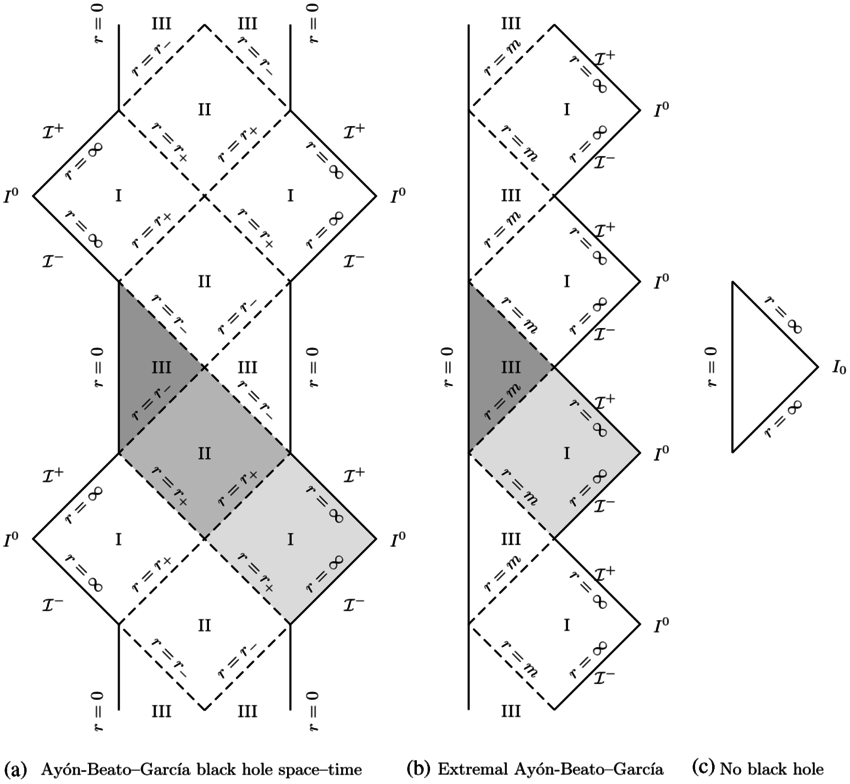
\includegraphics[scale=0.4]{GR/BH5.png}
\caption{Penrose diagram of RN spacetime}
\end{figure}

\section{Kerr black hole}
\subsection{Geometry of Kerr black hole}
The metric of Kerr black hole is
\[ds^2 = -\left(1 - \frac{2Mr}{\rho^2}\right)dt^2 - \frac{2Mar\sin^2\theta}{\rho^2}(dt d\phi + d\phi dt) + \frac{\rho^2}{\Delta} dr^2 + \rho^2d\theta^2 + \frac{\sin^2\theta}{\rho^2} \left[(r^2+a^2)^2 - a^2 \Delta \sin^2\theta\right]d\phi^2,\]
where
\[\Delta(r) = r^2 - 2Mr + a^2, \quad \rho^2(r,\theta) = r^2 + a^2 \cos^2\theta.\]
We can show that $a$ is the the angular momentum per unit mass of the black hole.
\\ \\
It is straightforward to check that as $a \to 0$ they reduce to Schwarzschild coordinates.
If we keep $a$ fixed and let $M \to 0$, we recover flat spacetime but not in ordinary polar coordinates. 
The metric becomes
\[ds^2 = -dt^2 + \frac{r^2+a^2\cos^2\theta}{r^2 + a^2} dr^2 + (r^2 + a^2\cos^2\theta)^2d\theta^2 + (r^2+a^2)\sin^2\theta d\phi^2,\]
and we recognize the spatial part of this as flat space in ellipsoidal coordinates. 
They are related to Cartesian coordinates in Euclidean $3$-space by
\begin{eqnarray}
x &=& (r^2+a^2)^{\frac{1}{2}} \sin\theta \cos\phi \nonumber \\
y &=& (r^2+a^2)^{\frac{1}{2}} \sin\theta \sin\phi \nonumber \\
z &=& r\cos\theta. \nonumber
\end{eqnarray}
$r = 0$ is a two-dimensional disk; the intersection of $r = 0$ with $\theta = \pi / 2$ is the ring at the boundary of this disk.
\\ \\
There are two Killing vectors of the metric, $K = \partial_t$ and $R = \partial_{\phi}$. The norms of these Killing vectors are scalar quantities with a coordinate-free, geometrical interpretation. 
This allows us to represent three of the metric coefficients in the form
\begin{eqnarray}
K^2 &=& g_{tt} = -\left( \frac{\Delta - a^2\cos^2\theta}{\rho^2} \right), \nonumber \\
K\cdot R &=& g_{t\phi} = \frac{a\sin^2\theta(\Delta - a^2 - r^2)}{\rho^2}, \nonumber \\
R^2 &=& g_{\phi\phi} = \frac{[(r^2+a^2)^2-\Delta a^2\sin^2\theta]\sin^2\theta}{\rho^2}. \nonumber
\end{eqnarray}
From the form of the Kerr metric, it is obvious that the metric becomes ill-defined at $\rho = 0$ and at $\Delta = 0$.
The calculation of scalar invariants of the curvature tensor shows that $\rho = 0$ is indeed a physical singularity. The condition $\rho = 0$ corresponds to
\[\rho^2 = r^2 + a^2\cos^2\theta = 0,\]
which can only be satisfied with $\theta = \pi/2$ and $r = 0$. Hence we have a ring-like singularity in the case of a Kerr metric. 
The curvature invariants are well behaved at $\Delta = 0$. 
$\Delta(r) = 0$ is equal to $g^{rr} = 0$. 
Thus $\Delta(r) = 0$ is a null surface.
The quadratic equation $\Delta = 0$ has two roots if $|a| < M$,
\[r_{\rm hor} = M \pm \sqrt{M^2-a^2},\]
representing inner and outer horizons in Kerr spacetime.
\\ \\
Let us consider the surface defined by the quadratic equation $g_{tt} = 0$. 
Consider a class of observers with four-velocity $u$ in the direction of the timelike Killing vector $K$. 
For any photon with four-momentum $p$ propagating in this spacetime, the observer with four-velocity $u$ will attribute a frequency
\[\omega = -p^{\mu}u_{\mu} =  \frac{p^{\mu}K_{\mu}}{K^{\mu}K_{\mu}} = \frac{E}{-g_{tt}}\]
where $E$ is the conserved ``energy'' of the photon. Thus it is easy to see that the surface with $g_{tt} = 0$ corresponds to infinite redshift.
For the Kerr metric, the equation $g_{tt}$ also has two solutions, $r = r_{\pm}$, given by
\[r_{\pm} = M \pm \sqrt{M^2-a^2\cos^2\theta}.\]
Physically, this corresponds to a surface of infinite redshift usually called an ergosurface.
The region between outer ergosurface and horizon is called the ergosphere.

\begin{figure}[!htb]
\centering
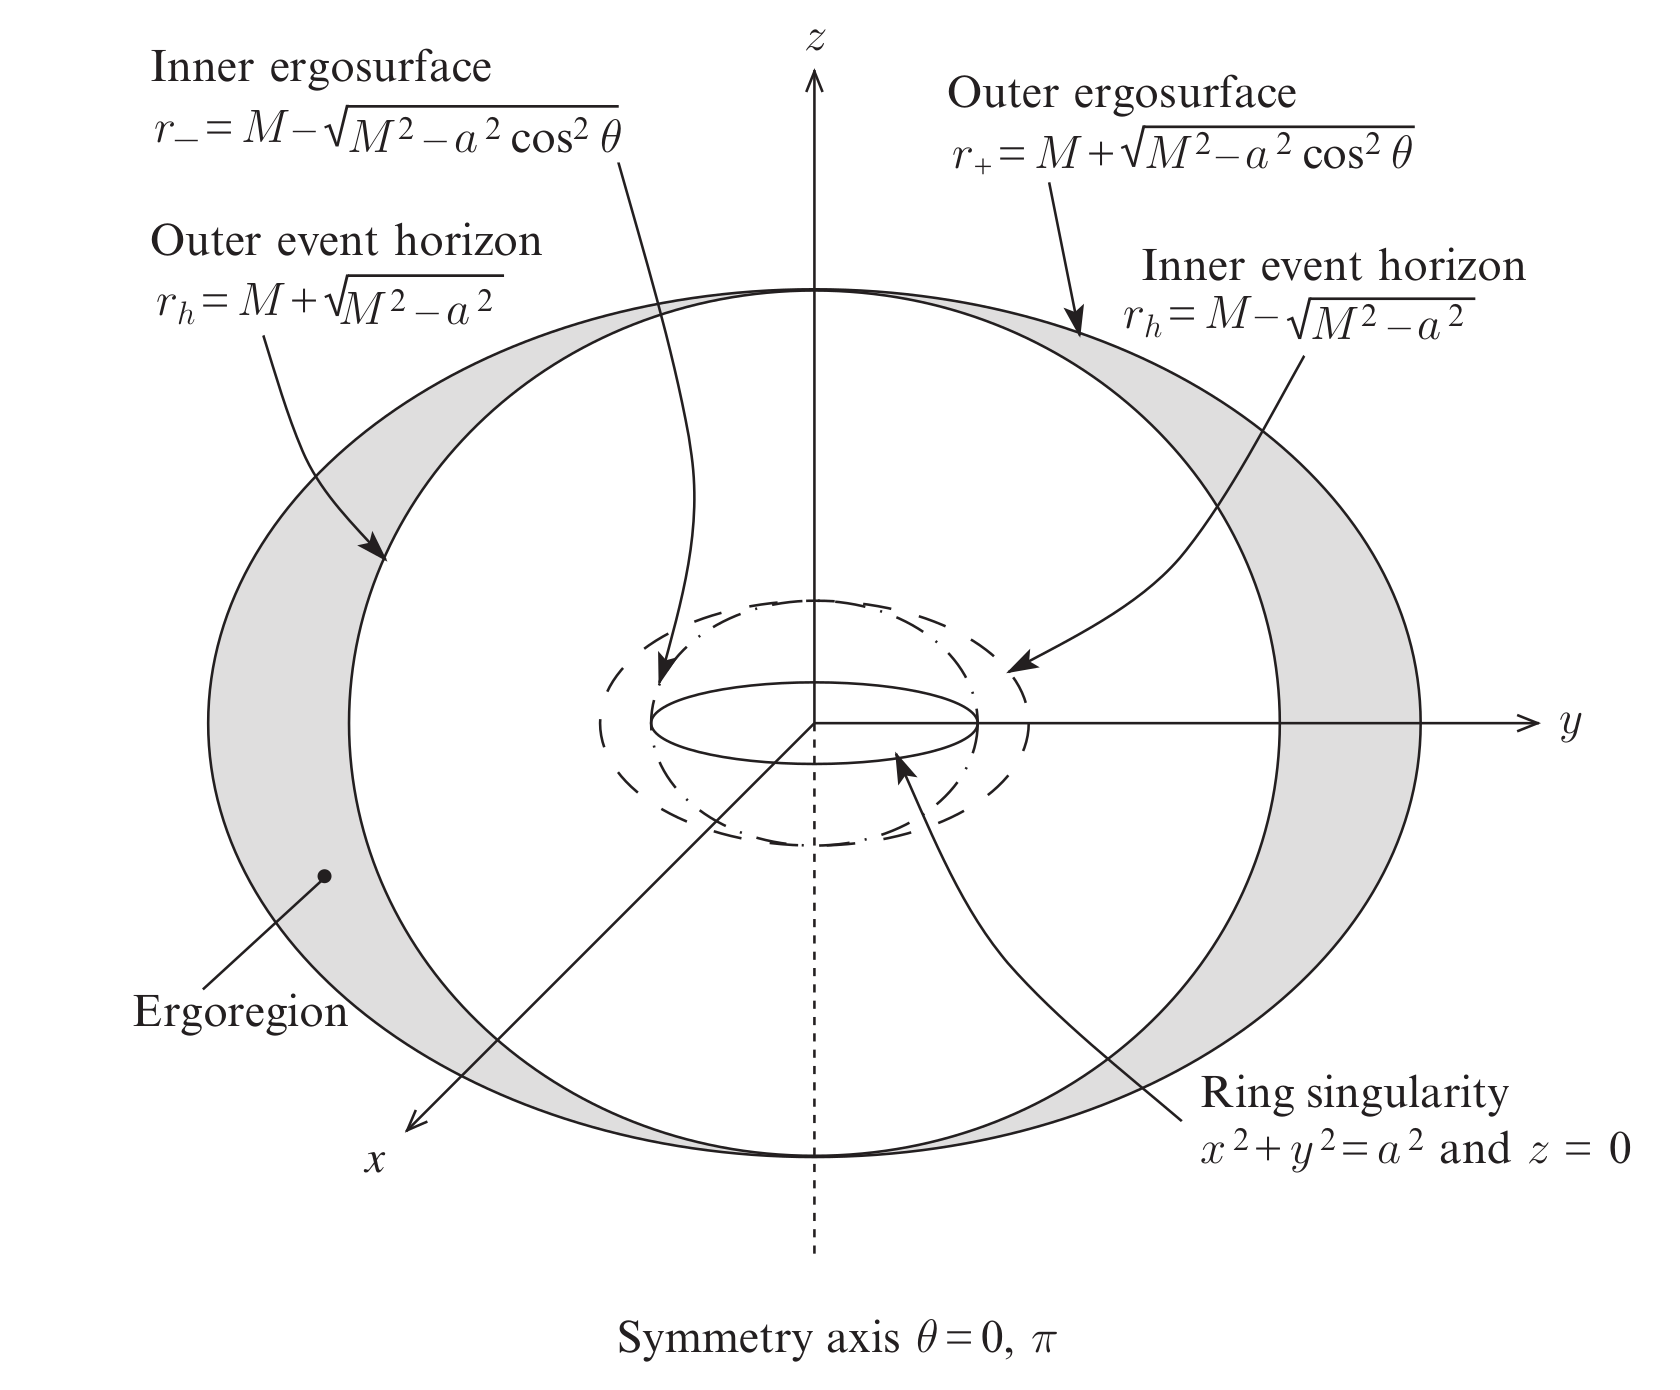
\includegraphics[scale=0.15]{GR/BH6.png}
\caption{Schematic picture showing the geometrical structure of the Kerr spacetime.}
\end{figure}

\begin{figure}[!htb]
\centering
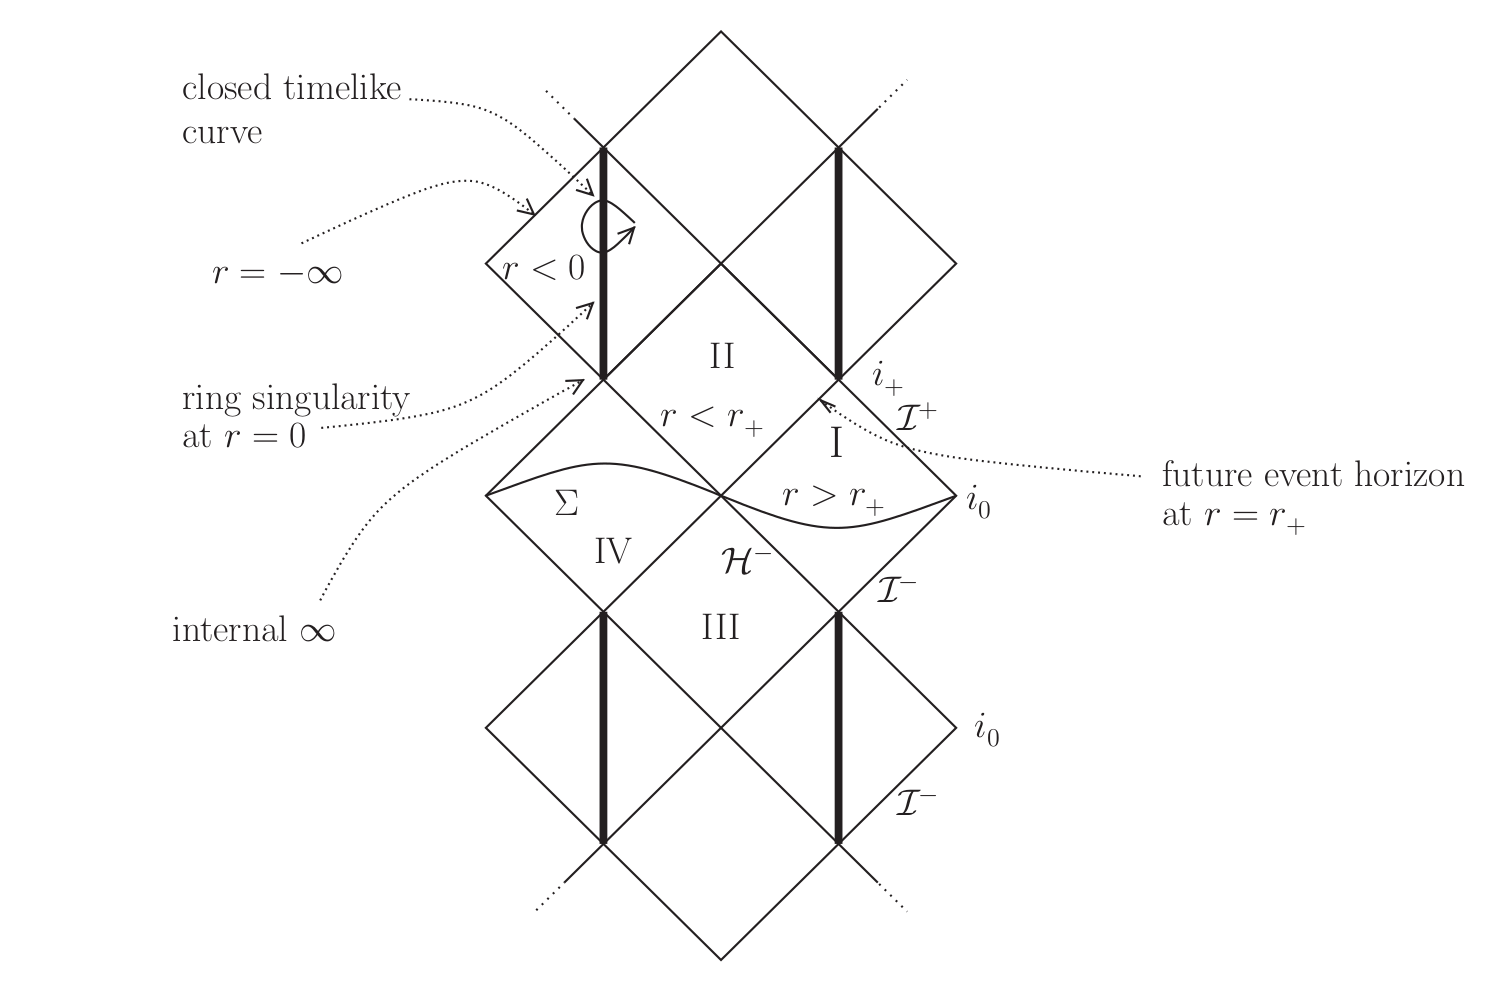
\includegraphics[scale=0.2]{GR/BH7.png}
\caption{The Penrose-Carter diagram for the Kerr spacetime for the case $M > a$.}
\end{figure}

\subsection{Static limit}
An observer in the Kerr spacetime moving with a constant angular velocity and having fixed values for $r$, $\theta$ will see the geometry to be unchanging. 
Such observers are called stationary observers. 
If the observers also have a fixed value for $\phi$, they are called static observers located at fixed spatial coordinates.
\\ \\
Consider a stationary observer with an angular velocity $\Omega$ in the Kerr spacetime with
\[\Omega = \frac{d\phi}{dt} = \frac{u^{\phi}}{u^{t}}.\]
Such an observer has a four-velocity $(u^{t},0,0,\Omega u^{t})$. From the normalization $u^{\mu}u_{\mu} = -1$, we have
\[g_{tt} + 2g_{t\phi}\Omega + g_{\phi\phi} \Omega^2 < 0.\]
This condition leads to limits in the range of values allowed for the angular velocity to be
\[\Omega_{\rm min} < \Omega < \Omega_{\rm max},\]
where
\[\Omega_{\rm min} = \omega - \sqrt{\omega^2 - (g_{tt}/g_{\phi\phi})}, \quad \Omega_{\rm max} = \omega + \sqrt{\omega^2 - (g_{tt}/g_{\phi\phi})},\]
with
\[\omega = -\frac{g_{\phi t}}{g_{\phi\phi}} = \frac{2Mar}{(r^2+a^2)^2-\Delta a^2\sin^2\theta}.\]
First, far away from the black hole, we have $r\Omega_{\rm min} = −1$ and $r\Omega_{\rm max} = +1$, which correspond to the standard result that motion should be at a speed less than that of light. 
Second, as one moves closer to the black hole, $\Omega_{\rm min}$ increases due to the dragging of the
inertial frames. 
Eventually, $\Omega_{\rm min}$ reaches zero at the surface on which $g_{tt} = 0$, which is the ergosurface. 
Therefore, inside the ergosphere, all stationary observers
must orbit the black hole with $\Omega > 0$ and hence static observers can exist only out-side the ergosurface. 
Finally, as one crosses the ergosurface and moves towards the event horizon, the allowed range of angular velocities become ever more positive with the allowed range narrowing down. 
At the event horizon, the $\Omega_{\rm min}$ and $\Omega_{\rm max}$ coincide and all timelike worldlines point inwards. 
The limiting angular velocity is given by
\[\Omega_{\rm H} \equiv \omega_{r_{\rm h},\theta} = \frac{a}{2Mr_{\rm h}}.\]
This limiting angular velocity is sometimes called the angular velocity of the horizon. Using this we can form a new Killing vector
\[K' \equiv K + \Omega_{\rm H} R.\]
It is clear that this Killing vector becomes null on the event horizon and is timelike outside the horizon.

\subsection{Penrose process and the area of the event horizon}
Since the Kerr metric has a timelike Killing vector field $K$ any particle moving on a geodesic will have a conserved energy given by $E = -P_{\mu} K^{\mu} = -p_{t}$.
We can derive that the orbit must be inside the ergosphere if the energy has to be negative.
\\ \\
This result can be used to extract energy from the Kerr black hole in several ways, of which the simplest one is the following. 
Consider, for example, a particle A moving in the ergosphere which breaks into two particles B and C. 
We let particle B to fall into the black hole and let particle C escape to infinity. 
All this can be done using suitable timelike trajectories. The conservation of four-momentum requires that
\[E_{\rm A} = E_{\rm B} + E_{\rm C}.\]
Since the particle A can fall into the ergosphere from infinity, we have $E_{\rm A} > m$.
We can arrange the trajectory of B making $E_{\rm B} < 0$. It immediately follows that $E_{\rm C} > E_{\rm A}$. 
When the particle C goes back to infinity, it will have more energy than the original particle had. 
Thus, using the existence of negative energy orbits in the ergosphere and the local conservation of energy for processes taking place in the ergo region, one can extract energy from the black hole.
\\ \\
The Penrose process decreases both the mass and the angular momentum of the Kerr black hole by an amount equal to the (negative of) the energy and the angular momentum of the particle B that falls into the black hole. 
Consider the dot product of $P^{\mu}$ with the Killing vector $K'$. 
Since $K'$ is timelike outside the horizon and we want particle B to fall into the horizon, it is necessary that this dot product is negative. 
Using $p^{\mu}K_{\mu} = -E$, $p^{\mu}R_{\mu} = L$,
where $E$ and $L$ are the conserved energy and angular momentum of particle B, we get the condition $-E + \Omega_{\rm H} L < 0$. 
When the particle B falls into the black hole, the angular momentum and mass of a Kerr black hole will change by $\delta J = L$ and $\delta M = E$. Hence the above bound
translates into the result
\[\delta M > \Omega_{\rm H} \delta J.\]
\\
The surface area of the event horizon of a Kerr black hole is given by
\[A = 4\pi (r_{\rm h}^2 + a^2).\]
We can verify that
\[\delta A = 8\pi \frac{a}{\Omega_{\rm H}\sqrt{M^2-a^2}}(\delta M - \Omega_{\rm H} \delta J).\]
This can be manipulated to read
\[\delta M = \frac{\delta \kappa}{8\pi G} \delta A + \Omega_{\rm H}\delta J,\]
where
\[\kappa = \frac{\sqrt{M^2-a^2}}{2M(M+\sqrt{M^2-a^2})}\]
is the surface gravity. 
Quantum field theory in curved space time would show that this relation can be given a thermodynamic interpretation with $\kappa / 2\pi$ acting as the temperature of the black hole and $A/4$ acting as the entropy of the black hole.

\subsection{Particle orbits in the Kerr metric}
The orbits of particles in the Kerr metric can be studied, in principle, by the same techniques we have used in the case of the Schwarzschild metric. 
However, lack of spherical symmetry makes the nature of the orbits very complicated and analytic solutions are impossible to find. 
It is clear that radial motion will now be possible only along the axis of symmetry and even planar motion will be possible only in the equatorial plane. 
Derivations of equations that govern the particle trajectories in the Kerr metric is given by subsection $8.5.4$ of \emph{Gravitation: Foundations and Frontiers ( T. Padmanabhan)}.
\\ \\
The existence of stable circular orbits in the equatorial plane is of some practical interest in astrophysics. 
It is generally believed that the matter in the accretion
disks around astrophysical black holes will be able to move towards the black hole in a series of approximately circular orbits in the equatorial plane. 
In that case, the radius of the stable circular orbit closest to the black hole and its energy are
of interest in the astrophysics of accretion disks. 
For the motion in the equatorial plane one can introduce an effective potential as in the case of the Schwarzschild
metric along the following lines. Setting $\theta = \frac{\pi}{2}$ into equations of motion will give equation for the radial motion,
\[m^2 \left(\frac{dr}{d\tau} \right)^2 = \frac{[(r^2+a^2)E-aL]^2}{r^4} - \frac{\Delta[(aE-L)^2+m^2 r^2]}{r^4}.\]
We can now define an effective $U(r)$ such that the right hand side of the above equation vanishes when $E=U$. 
Hence the effective potential is the solution to the
equation:
\[[(r^2+a^2)U(r)-aL]^2 - \Delta[(aU(r)-L)^2+m^2 r^2] = 0.\]
The radii of stable circular orbits are determined by the minima of $U(r)$; that is by the simultaneous solution to the equations $E = U(r)$, $U'(r) = 0$. 
Among all the stable circular orbits, we are interested in the innermost one. 
Fairly lengthy but straightforward calculation shows that this orbital radius is the solution to the quartic equation
\[r^2 - 6Mr - 3a^2 \mp 8a\sqrt{Mr} = 0,\]
where the upper (lower) sign corresponds to the counter-rotating (co-rotating) orbit.
When $a = 0$ we get the standard result that $r = 6M$; as the rotation parameter increases, the radius of the circular orbit decreases for the co-rotating orbit which is the one that is probably the relevant one for the accretion disk. 
This shows that one can have stable circular orbits very
close to the black hole in the case of rotating black holes. 
The quantity $(m − E)/m$ represents the fraction of the rest energy that can be released when a particle falls from the innermost stable circular orbit into the black hole. 
In the extreme case of $a = M$, this fraction is $1 - 1 / \sqrt{3}$ which is about $42$ percent, while the corresponding value for orbits in the Schwarzschild metric is only about $5.7$ percent. 
This higher efficiency could be of use in certain astrophysical scenarios.

\chapter{Geometry of the Universe}
\section{Friedmann–Lemaître–Robertson–Walker metric}
The metric in standard model of cosmology is
\[ds^2 = -dt^2 + a(t)^2 \left(\frac{dr^2}{1-Kr^2} + r^2 d\Omega^2 \right).\]
If we define
\[\chi \equiv \begin{cases} 
\sin^{-1}(\sqrt{K}r)/\sqrt{K}, K > 0 \\
r, K = 0 \\
\sinh^{-1}(\sqrt{-K}r)/\sqrt{-K}, K < 0
\end{cases}\]
and
\[\eta \equiv \int \frac{dt}{a(t)},\]
the metric can then be written as
\[ds^2 =  a(\eta)^2 \left(-d\eta^2 + d\chi^2 + r(\chi)^2 d\Omega^2 \right).\]
In coordinates $(t,r,\theta,\phi)$, we have
\[G_{tt} = \frac{3(\dot{a}^2+K)}{a^2}, \quad G^{\mu}_{\mu} = -\frac{6(\dot{a}^2+a\ddot{a}+K)}{a^2}.\]  
Suppose that the matter in the universe can be modelled as idealized fluid. Thus the corresponding energy-momentum tensor is $T^{\mu\nu} = (\rho + p) u^{\mu} u^{\nu} + pg^{\mu\nu}$. Contraction of the energy-momentum tensor gives $T^{\mu}_{\mu} = -\rho + 3p$. 
If the matter is comoving with the coordinates, we have $T_{tt} = \rho$. Einstein equations now takes the from as
\[\left(\frac{\dot{a}}{a} \right)^2 = \frac{8\pi}{3}\rho - \frac{K}{a^2}, \quad \frac{\ddot{a}}{a} = - \frac{4\pi}{3}(\rho + 3p),\]
called Friedmann equations. If we take the derivative of the first equation, we can get
\[\frac{\ddot{a}}{a} = -\frac{4\pi}{3}\left( - \frac{d\rho}{d \ln a} -2\rho \right).\]
By comparing with the second equation, we have
\[\frac{d\rho}{d \ln a} = -3(p+\rho).\]
If we have the equation of state $p = k\rho$, then it is easy to verify that $\rho \propto a^{-3(k+1)}$.
As for radiation (photon), we have $p_{\rm R} = 1/3 \rho_{\rm R}$, so $\rho_{\rm R} \propto a^{-4}$. As for cold matters (baryon, cold dark matter), we have $p_{\rm CM} = 0$, so $\rho_{\rm CM} \propto a^{-3}$. As for dark energy, we have $p_{\rm DE} = - \rho_{\rm DE}$, so $\rho_{\rm DE} = $ constant. Our universe is mainly composed of dark energy, cold dark matters, baryons and radiations. 
The Friedmann equations can be now written as
\[\frac{H^2}{H_0^2} = \Omega_{\rm R0}a^{-4} + \Omega_{\rm CM0} a^{-3} + \Omega_{\rm DE0} + \Omega_{\rm K0}a^{-2}.\]
In equation above, the subscript $0$ denotes today's value of some parameters and we scale the coordinates to make $a_0 = 1$. 
$H \equiv \dot{a} / a$ and $H_0$ is called Hubble's constant. $\Omega_0$ is the ratio between density $\rho_0$ of some substance and critical density $\rho_{\rm c0} \equiv \frac{3H_0^2}{8\pi}$. Particularly, $\rho_{\rm K0} = 3K/8\pi$ is called the density of curvature energy and we can note that $\Omega_{\rm K0} = 1 - \Omega_{\rm DE0} - \Omega_{\rm CM0} - \Omega_{\rm R0}$.

\section{Observable quantities}
\subsubsection{Redshift}
Suppose there is a photon emitted from $r=0$ at time $t$, then the world line of the photon will satisfy that
\[\left(\frac{dt}{dr}\right)^2 = \frac{a^2}{1-Kr^2}, \quad \theta = \mbox{ Constant}, \quad \phi = \mbox{ Constant}.\]
In terms of four-momentum, we have
\[\left(\frac{p^t}{p^r}\right)^2 = \frac{a^2}{1-Kr^2}\]
On the other hand, we have the geodesic equation that
\[\frac{dp^{t}}{d\lambda} + \Gamma^{t}_{\phantom{*}\alpha \beta} p^{\alpha}p^{\beta} = \frac{dp^{t}}{d\lambda} + \frac{a\dot{a}}{1-Kr^2}(p^r)^2 = 0.\]
It can be simplified to
\[\frac{dp^t}{p^t} + \frac{da}{a} = 0.\]
Note that $a_0 = 1$, so we have $p^t_0 = ap^t$. Define cosmological redshift by $p_0^t = p^t/(1+z)$. We have the relation
\[a = \frac{1}{1+z}.\]

\subsubsection{Luminosity}
Suppose there is an object with intrinsic luminosity $L$ at $r = 0$ and time $t$. Suppose at time $t_0$, the photon propagate to $r = r_0$(our position) at time $t_0$ (now). In coordinates $(\eta,\chi)$, we have $\eta_0 = \chi_0$. Thus
\[\chi_0(z) = \int_{t}^{t_0} \frac{dt'}{a} = \int_{0}^{z} \frac{dz'}{H(z')},\]
where $z$ is the redshift of the object and 
\[r_0 \equiv \begin{cases} 
\sin(\sqrt{K}\chi_0)/\sqrt{K}, K > 0 \\
\chi_0, K = 0 \\
\sinh(\sqrt{-K}\chi_0)/\sqrt{-K}, K < 0.
\end{cases}\]
The area size of the two surface $t=t_0$, $r=r_0$ is $4\pi r_0^2$. In time interval $\Delta t$, the object emitted $\Delta N$ photons, then we have $L = \epsilon \Delta N / \Delta t$. $\epsilon$ is the energy of the photon.
The interval for receiver is $\Delta t_0 = \Delta t / a$ (It is easy to verify in coordinates $(\eta,\chi)$ that $\Delta \eta = \Delta \eta'$). Take into account the redshift of the photon, the flux we measured is
\[f = \frac{\epsilon \Delta N}{(1+z)\Delta t_0 4\pi r_0^2} = \frac{L}{4\pi d_{\rm L}^2},\]
where $d_{\rm L} = (1+z)r_0$.

\subsubsection{Size}
Suppose there is an object with intrinsic size $\Delta l$ at time $t$. Now we put ourselves at $r = 0$, so the object will be at the two surface with metric $d\sigma^2 = a(t)^2 r_0^2 d\Omega^2$. The angle it extends relative to us satisfy that $ar_0\Delta\theta = \Delta l$, i.e.
\[\Delta \theta = \frac{\Delta l}{d_{\rm A}},\]
where $d_{\rm A} = r_0/(1+z)$.